\chapter{Sampling} \label{ch:sampling}

There is an important underlying assumption in statistics: the features observed from measurements or samples can somehow reflect the features of the ``truth''. In this context, ``truth'' could mean unknown parameters in a parameter estimation problem, unknown states in a state estimation problem, or statistics features of the large size population. 

Parameter and state estimation problems are covered in other control-related notebooks. The main focus of this section the the following sections are the deriving of statistics features of the population using the samples. Statistics is helpful with at least the following:
\begin{itemize}
	\item Selection of samples,
	\item Derive statistics features of the population from the samples,
	\item Analysis of the accuracy and reliability of the derived statistics features.
\end{itemize}

\section{Sampling Methods}

When selecting elements from the population, make sure that all elements have a equal probability of being selected, hence, random sampling. Depending on whether an element can be selected multiple times, we have
\begin{itemize}
  \item Sampling with replacement: a member can be chosen more than once.
  \item Sampling without replacement: a member can be chosen no more than once.
\end{itemize}

Sometimes it is interesting to compare the differences of the two methods, especially when the population is finite. An obvious difference is that by using sampling with replacement all the samples can be considered as ``independent event''. In this case, using sampling with replacement can theoretically be considered as sampling from an infinite population by thinking that the population is duplicated as many times as necessary. While by using sampling without replacement, previous samples may change the distributions in the remaining samples in the population, thus making the samples relevant. In practice, the population is usually so large and the two methods would make no differences as far as it is concerned.

For further demonstration of the differences between sampling with and without replacement, consider the following example. A set of $N$ random variables are generated from a Gaussian distribution as the population. Sample the population $M$ times using sampling with/without replacement. Calculate the sampled mean and variance after each sampling instance, and see how it converges to the mean and variance of the population.

In the first example, let $N=100$ and $M=500$. Figures \ref{ch:sampling:fig:sample-wr-n100} and \ref{ch:sampling:fig:sample-nwr-n100} gives the cumulative mean and variance of sampling with and without replacement, respectively. The mean and variance are given by red and blue curves, respectively. The statistics obtained from the cumulative samples and from the population are given by the solid and dashed curves, respectively. Notice that in Fig. \ref{ch:sampling:fig:sample-nwr-n100}, after number of samples exceeding $100$, the entire population has been sampled, and thus the sampling stops. This explains why its mean and variance stop fluctuating and converge to the population mean and variance respectively.

\begin{figure}
	\centering
	\includegraphics[width=250pt]{chapters/ch-sampling/figures/sample-wr-n100.eps}
	\caption{Sample with replacement, population size $N=100$, sample size $0< M\leq500$.} \label{ch:sampling:fig:sample-wr-n100}
\end{figure}

\begin{figure}
	\centering
	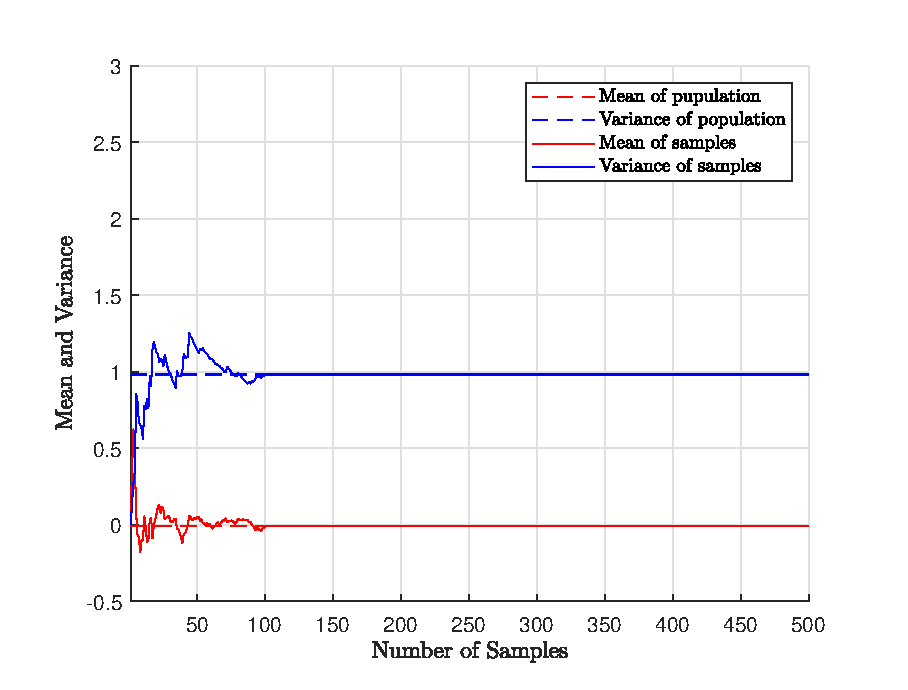
\includegraphics[width=250pt]{chapters/ch-sampling/figures/sample-nwr-n100.eps}
	\caption{Sample without replacement, population size $N=100$, sample size $0< M\leq500$.} \label{ch:sampling:fig:sample-nwr-n100}
\end{figure}

In practice, however, the population size is often orders of magnitudes larger than the number of samples. In the second example, let $N=10000$ and $M=500$. The corresponding figures are given in Figs. \ref{ch:sampling:fig:sample-wr-n10000} and \ref{ch:sampling:fig:sample-nwr-n10000}. There is no obvious differences of the two figures.

\begin{figure}
	\centering
	\includegraphics[width=250pt]{chapters/ch-sampling/figures/sample-wr-n10000.eps}
	\caption{Sample with replacement, population size $N=10000$, sample size $0< M\leq500$.} \label{ch:sampling:fig:sample-wr-n10000}
\end{figure}

\begin{figure}
	\centering
	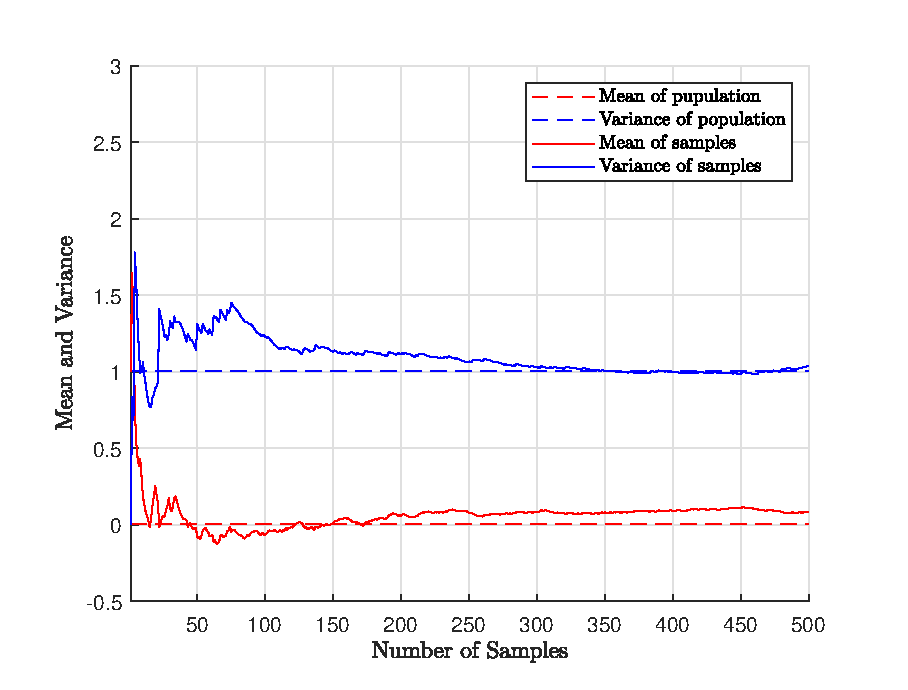
\includegraphics[width=250pt]{chapters/ch-sampling/figures/sample-nwr-n10000.eps}
	\caption{Sample without replacement,population size $N=10000$, sample size $0< M\leq500$.} \label{ch:sampling:fig:sample-nwr-n10000}
\end{figure}

\section{Model of Population}

The features of the population is often unknown, or at least not known precisely. It is possible to make some preliminary assumptions to the distribution. The samples are then used to consolidate or reject the assumptions.

For example, let $X$ be a feature of the population. It could be, for example, the heights of all teenagers in a city. We can make an assumption that $X$ follows Gaussian distribution with mean $\mu$ and standard deviation $\sigma$, and each element in the population, $X_i$, can be taken as a random variable generated from $f(x)$.

The objective it to use the samples to answer the following questions:
\begin{itemize}
  \item Does it indeed follow the assumed distribution, in this example, Gaussian distribution?
  \item What are the parameters of the assumed distribution, in this example, $\mu$ and $\sigma$?
\end{itemize}

\section{Sample Statistics}





